%%%%%%%%%%%%%%%%%%%%%%%%%%%%%%%%%%%%%%%%%
% Beamer Presentation
% LaTeX Template
% Version 1.0 (10/11/12)
%
% This template has been downloaded from:
% http://www.LaTeXTemplates.com
%
% License:
% CC BY-NC-SA 3.0 (http://creativecommons.org/licenses/by-nc-sa/3.0/)
%
%%%%%%%%%%%%%%%%%%%%%%%%%%%%%%%%%%%%%%%%%

%----------------------------------------------------------------------------------------
%	PACKAGES AND THEMES
%----------------------------------------------------------------------------------------

\documentclass{beamer}

\mode<presentation> {

% The Beamer class comes with a number of default slide themes
% which change the colors and layouts of slides. Below this is a list
% of all the themes, uncomment each in turn to see what they look like.

%\usetheme{default}
%\usetheme{AnnArbor}
%\usetheme{Antibes}
%\usetheme{Bergen}
%\usetheme{Berkeley}
%\usetheme{Berlin}
%\usetheme{Boadilla}
%\usetheme{CambridgeUS}
%\usetheme{Copenhagen}
%\usetheme{Darmstadt}
%\usetheme{Dresden}
%\usetheme{Frankfurt}
%\usetheme{Goettingen}
%\usetheme{Hannover}
%\usetheme{Ilmenau}
%\usetheme{JuanLesPins}
%\usetheme{Luebeck}
\usetheme{Madrid}
%\usetheme{Malmoe}
%\usetheme{Marburg}
%\usetheme{Montpellier}
%\usetheme{PaloAlto}
%\usetheme{Pittsburgh}
%\usetheme{Rochester}
%\usetheme{Singapore}
%\usetheme{Szeged}
%\usetheme{Warsaw}

% As well as themes, the Beamer class has a number of color themes
% for any slide theme. Uncomment each of these in turn to see how it
% changes the colors of your current slide theme.

%\usecolortheme{albatross}
\usecolortheme{beaver}
%\usecolortheme{beetle}
%\usecolortheme{crane}
%\usecolortheme{dolphin}
%\usecolortheme{dove}
%\usecolortheme{fly}
%\usecolortheme{lily}
%\usecolortheme{orchid}
%\usecolortheme{rose}
%\usecolortheme{seagull}
%\usecolortheme{seahorse}
%\usecolortheme{whale}
%\usecolortheme{wolverine}

%\setbeamertemplate{footline} % To remove the footer line in all slides uncomment this line
%\setbeamertemplate{footline}[page number] % To replace the footer line in all slides with a simple slide count uncomment this line

%\setbeamertemplate{navigation symbols}{} % To remove the navigation symbols from the bottom of all slides uncomment this line
}

\usepackage{graphicx} % Allows including images
\usepackage{booktabs} % Allows the use of \toprule, \midrule and \bottomrule in tables
\usepackage[francais]{babel}
\usepackage[utf8]{inputenc}
%----------------------------------------------------------------------------------------
%	TITLE PAGE
%----------------------------------------------------------------------------------------

\title[Sentiment analysis with RNN]{Analyse de sentiment par réseaux neuronaux réccurents} % The short title appears at the bottom of every slide, the full title is only on the title page

\author{Bertrand Rondepierre \& Thomas Moreau} % Your name
\institute[] % Your institution as it will appear on the bottom of every slide, may be shorthand to save space
{
Télécom paristech - MDI343 \\
}
\date{\today} % Date, can be changed to a custom date

\begin{document}

\begin{frame}
\titlepage % Print the title page as the first slide
\end{frame}

\begin{frame}
\frametitle{Overview} % Table of contents slide, comment this block out to remove it
\tableofcontents % Throughout your presentation, if you choose to use \section{} and \subsection{} commands, these will automatically be printed on this slide as an overview of your presentation
\end{frame}

%----------------------------------------------------------------------------------------
%	PRESENTATION SLIDES
%----------------------------------------------------------------------------------------

%------------------------------------------------
\section{Analyse de sentiment} % Sections can be created in order to organize your presentation into discrete blocks, all sections and subsections are automatically printed in the table of contents as an overview of the talk
%------------------------------------------------

\subsection{Les objectifs}

%------------------------------------------------

\begin{frame}
\frametitle{Les Objectifs}
\begin{itemize}\setlength{\itemsep}{5mm}
\item Catégoriser l'opinion général exprimer par une phrase
\item Plusieurs niveaux (analyse binaire / fine)
\item Représenter la phrase dans un espace propre qui permettre de mettre en lumière l'opinion qu'elle contient
\item Généré des phrases?
\end{itemize}
\end{frame}

%------------------------------------------------

\begin{frame}
\frametitle{Le Stanford Tree bank}
\begin{itemize}\setlength{\itemsep}{5mm}
\item 11 855 critiques de film
\item Labels et structure de la phrase sous forme d'arbre\\
$\Rightarrow$ Possibilité d'analyse fine à chaque noeuds
\end{itemize}

\begin{figure}[htp]
\centering
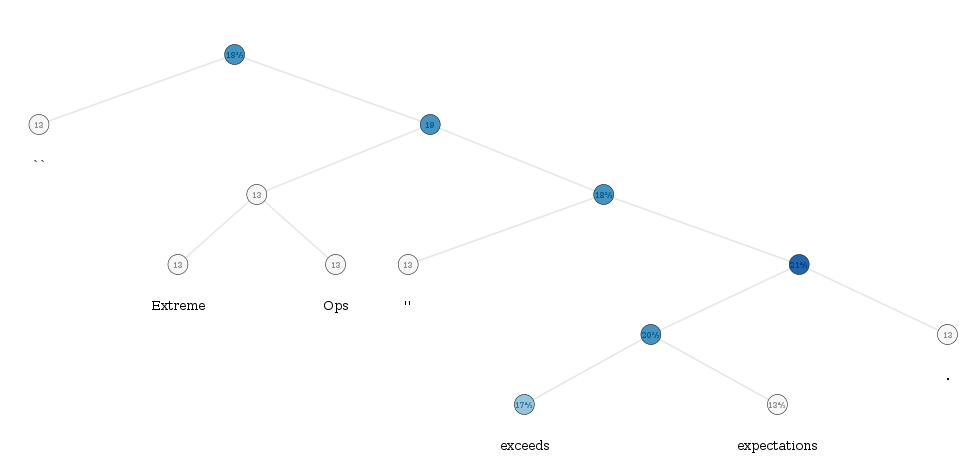
\includegraphics[scale=0.2]{fig/Tree10.png}
\caption{"Extreme Ops" exceeds expectations.}
\end{figure}

\end{frame}

%------------------------------------------------

\begin{frame}
\frametitle{Le model}
\begin{itemize}\setlength{\itemsep}{7mm}
\item \textbf{Classique}: Bag of words 
\item N'analyse pas la structure de la phrase (négation, expression)\\
\emph{This movie was actually neither that funny, nor super witty.}
\item L'idée est d'utiliser la structure d'arbre pour predire le sentiment de la phrase.
\item On cherche aussi a optimiser la représentation des mots
\end{itemize}

\end{frame}

%------------------------------------------------
\section{L'apprentissage du model}

\begin{frame}
\frametitle{Fonction de cout}
\begin{itemize}\setlength{\itemsep}{7mm}
\item $ \displaystyle   E = \sum_{phrase}\sum_{nodes} t_i \log y_i$.
\item Dans le papier, met les labels en dimension 5\\
$\Rightarrow$ suppose equi distance entre les labels
\item Notre approche: regression et attribution d'un label avec une frontière fixe.
\end{itemize}
\end{frame}

%------------------------------------------------

\begin{frame}
\frametitle{Apprentissage}
\begin{itemize}\setlength{\itemsep}{7mm}
\item Calcul du gradient par back propagation
\begin{align*}
	\frac{\partial E}{\partial \theta} = \frac{t_i}{y_i} F'(y_i)\left[\frac{\partial W}{\partial \theta}x_{i-1} + \frac{\partial V}{\partial \theta} x_{i-1}x_{i-1}^T + \left( 2 V x_{i-1} + W  \right) \frac{\partial x_{i-1}}{\partial \theta} \right]
\end{align*}
\item Notre model implémente Ada-grad \\
$\Rightarrow$ Principe est de réduire le learning rate des poids qui ont déja beaucoup été updaté.
\item Autre solution: Rms prop\\
$\Rightarrow$ On tune le learning rate en fonction de la dynamique du gradient.
\end{itemize}
\end{frame}

%------------------------------------------------
\section{Les résultats }

\begin{frame}
\frametitle{Paramètre}
\begin{itemize}
\item Learning rate, mini batch size, regularisation
\end{itemize}
\begin{figure}[htp]
\centering
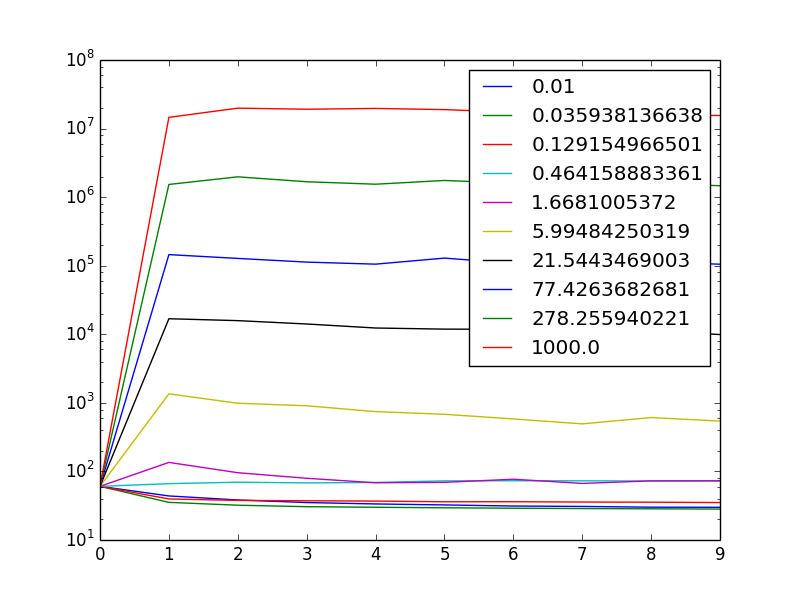
\includegraphics[scale=0.2]{fig/lr_curves.png}
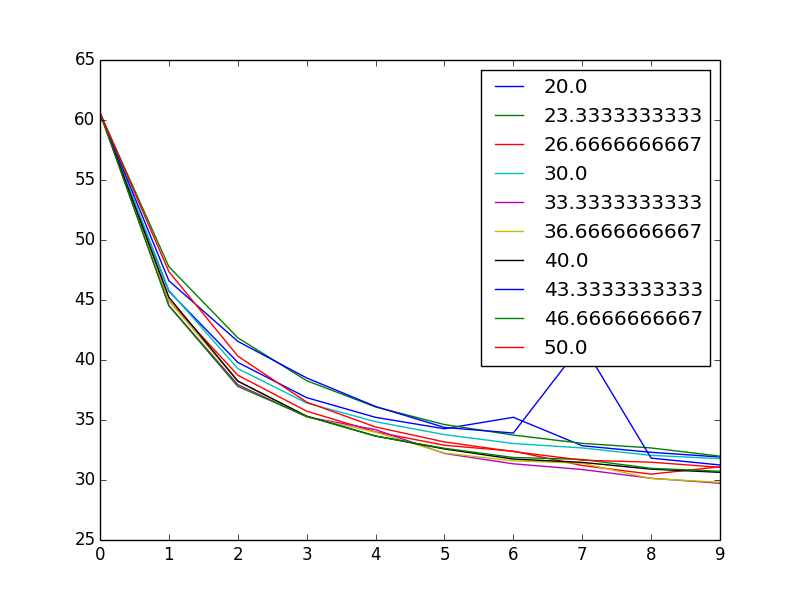
\includegraphics[scale=0.2]{fig/mb_curves.png}
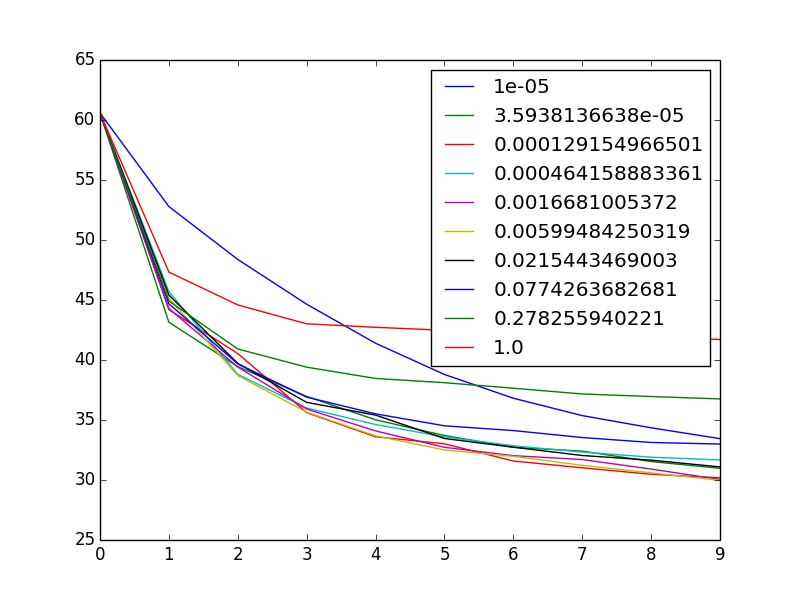
\includegraphics[scale=0.2]{fig/reg_curves.png}
\caption{Courbe d'apprentisssage en Cross validation pour le learning rate, la taille du mini batch et le facteur de régularisation}
\end{figure}

\end{frame}

%------------------------------------------------

\begin{frame}
\frametitle{Apprentissage}
\begin{figure}[htp]
\centering
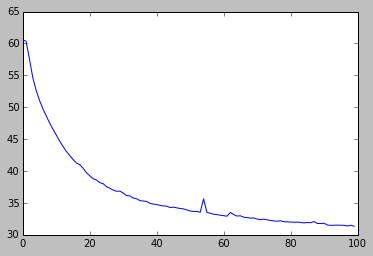
\includegraphics[scale=0.4]{fig/CourbeValAdaGrad.png}
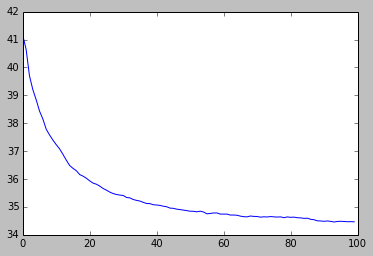
\includegraphics[scale=0.4]{fig/CourbeValRprop.png}
\caption{Courbe d'apprentisssage pour AdaGrad \emph{(gauche)} et Rprop \emph{(droite)}}
\end{figure}

\end{frame}

%------------------------------------------------

\begin{frame}
\frametitle{Resultat de Classification}
\begin{center}
\begin{tabular}{| c | c | c | c | c |}
\cline{2-5}
\multicolumn{1}{c}{} & \multicolumn{2}{| c |}{Fine} & \multicolumn{2}{| c |}{Binaire}\\\cline{2-5}
\multicolumn{1}{c |}{} & All node & Root & All nodes & Root \\\hline
Socher & 80.7  & 45.7 & 87.6 & 85.4\\\hline
Notre modèle & 79.7 & 42.2  & 86.6 & 90.6\\\hline
\end{tabular}
\end{center}

\begin{figure}[htp]
\centering
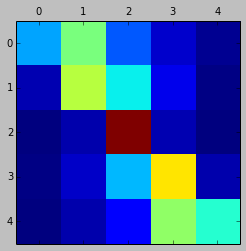
\includegraphics[scale=0.5]{fig/CMLastTrain.png}
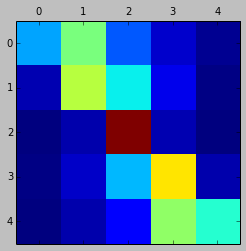
\includegraphics[scale=0.5]{fig/CMLastTrain.png}
\caption{Matrice de confusion \emph{(gauche)} Noeuds \emph{(droite)} Root}
\end{figure}

\end{frame}

%------------------------------------------------

\begin{frame}
\frametitle{Resultat de Classification}

\begin{figure}[htp]
\centering
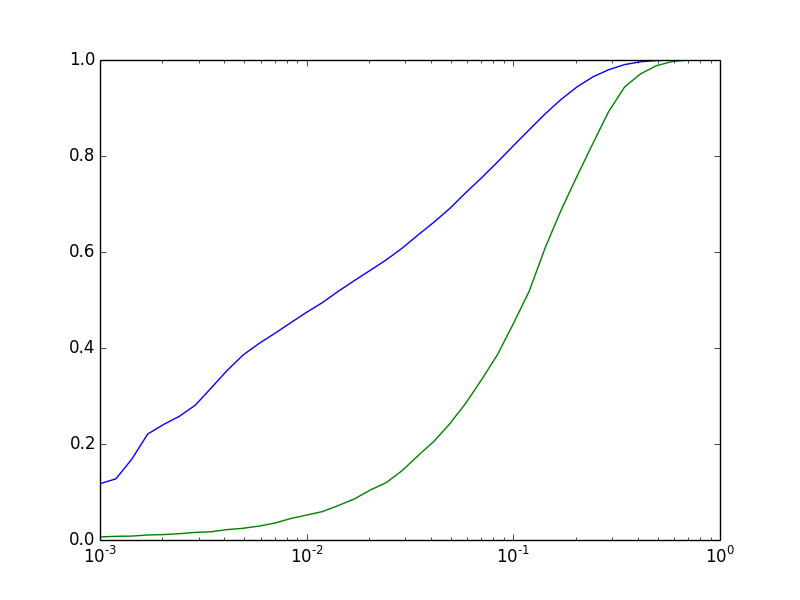
\includegraphics[scale=0.4]{fig/log_eps_curve.png}
\caption{Precision de notre regression (log scale)}
\end{figure}

\end{frame}


%------------------------------------------------

\begin{frame}
\frametitle{Representation apprise - Mots}
\begin{figure}[htp]
\centering
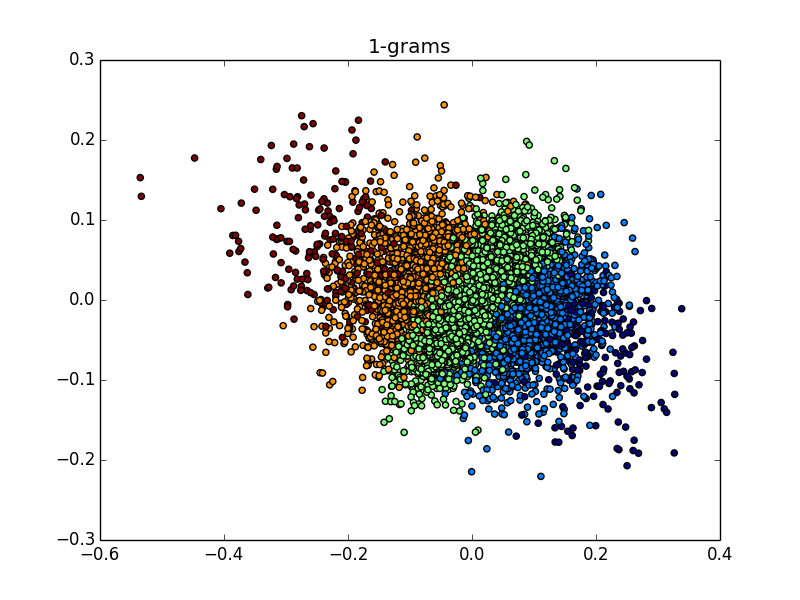
\includegraphics[scale=0.25]{fig/WordPlot1.png}
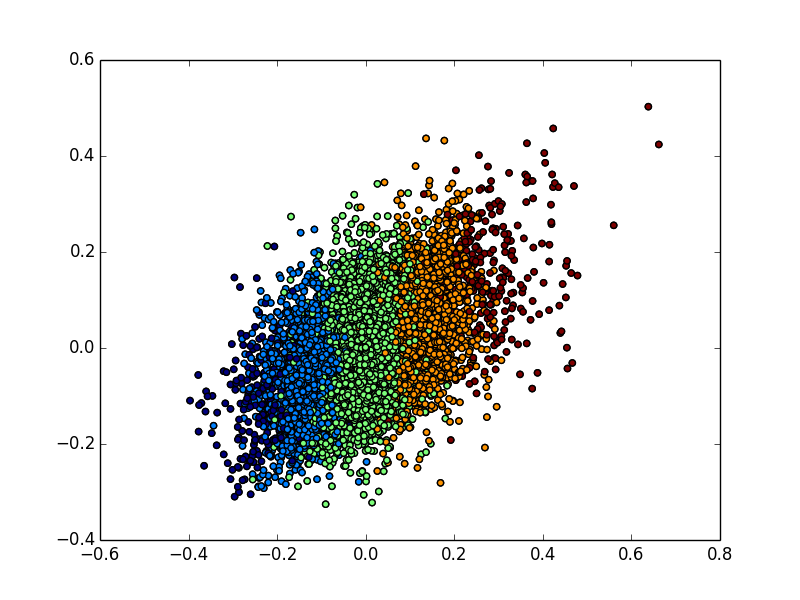
\includegraphics[scale=0.25]{fig/model2d.png}

\caption[caption]{PCA de la representation des mots en dimension 2. \hspace{\textwidth}.\hspace{0.1\textwidth}\emph{(gauche)} PCA sur modèle 30D \emph{(droite)} modèle 2D}
\end{figure}

\end{frame}
%------------------------------------------------

\begin{frame}
\frametitle{Representation apprise - N-grams}
\begin{figure}[htp]
\centering
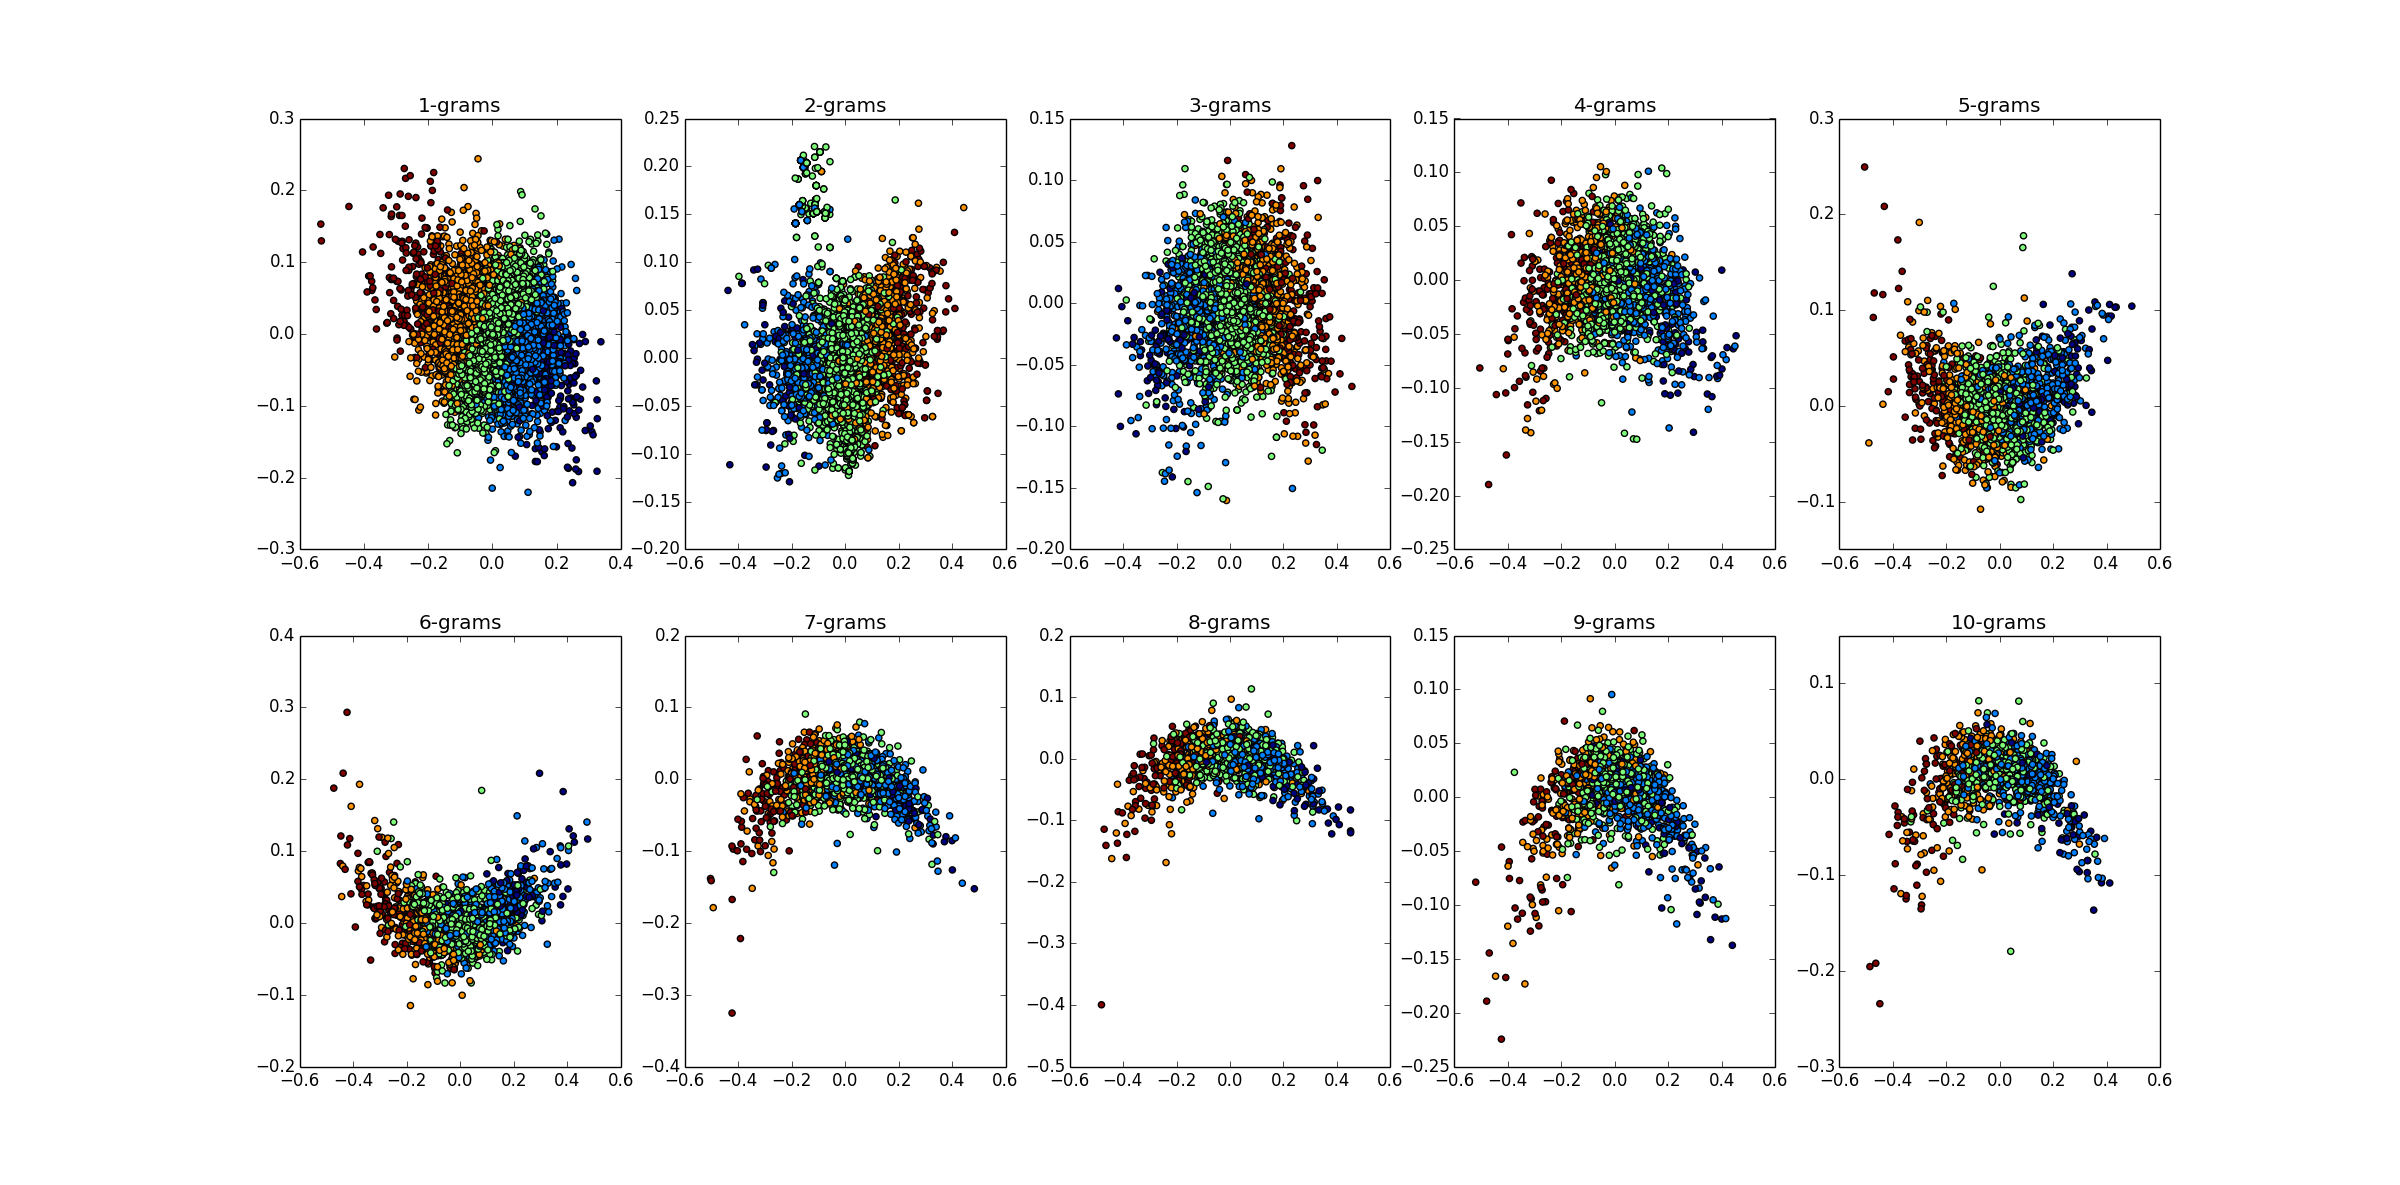
\includegraphics[scale=0.2]{fig/n_gram.png}
\caption[caption]{PCA de la representation des mots en dimension 2 pour le modèle 30d}
\end{figure}

\end{frame}

%------------------------------------------------

\section{Auto encoder}
\begin{frame}
\frametitle{Auto encoder?}
\begin{itemize}
\item L'idée est que l'on combine mal les représentations.
\item Auto encoder optimize la reconstruction\\
$\Rightarrow$ Meilleur prise en compte de l'information?
\item L'idée du modèle est
\begin{figure}[htp]
\centering
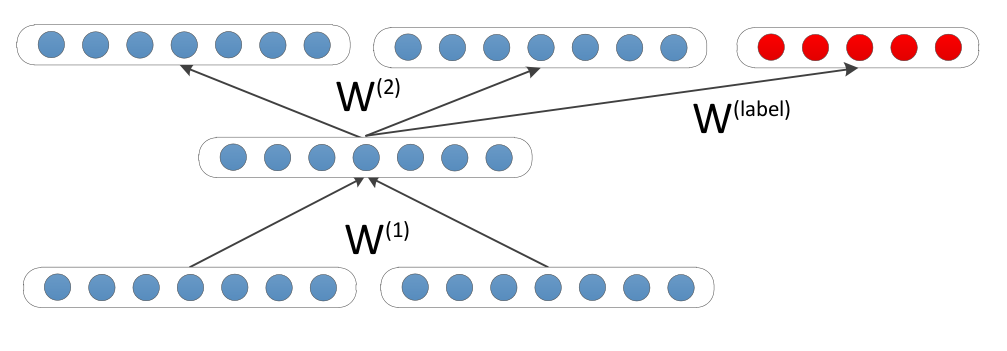
\includegraphics[scale=0.2]{fig/model_RAE.png}
\label{}
\end{figure}
\end{itemize}
\end{frame}

%------------------------------------------------

\begin{frame}
\frametitle{So far...}
\begin{itemize}\setlength{\itemsep}{5mm}
\item Back propagation découle de celle de notre modèle précédent
\item Ajout d'une dimension pour le sampling
\item Pour le moment, pas de structure, mais du sentiment.
\end{itemize}
\end{frame}


%------------------------------------------------

\begin{frame}
\Huge{\centerline{Question ?}}
\end{frame}

%----------------------------------------------------------------------------------------

\end{document} 